\documentclass[10pt,t]{beamer}

\usepackage[utf8]{inputenc}
\usepackage[T1]{fontenc}
\usepackage{graphicx}
\usepackage{grffile}
\usepackage{longtable}
\usepackage{wrapfig}
\usepackage{rotating}
\usepackage[normalem]{ulem}
\usepackage{amsmath}
\usepackage{textcomp}
\usepackage{amssymb}
\usepackage{capt-of}
\usepackage{hyperref}

\input beamer_setup

\usetheme{default}
% ---------------------------------------------------------------------
% ---------------------------------------------------------------------
\begin{document}

\title[]{15 years of Longwave Flux Trends : \newline
  Roles of CO2, WV, Temperature and clouds, \newline
  using ERA and AIRS data}
\author{Sergio DeSouza-Machado, Larrabee Strow}
\institute{Department of Physics, JCET\\
  University of Maryland Baltimore County (UMBC)}
\date{October 2, 2018}
% ---------------------------------------------------------------------
% ---------------------------------------------------------------------
\begin{frame}
  \titlepage
\end{frame}
% ---------------------------------------------------------------------
\begin{frame}
  \frametitle{Overview}
  \begin{itemize}
  \item CERES can produce total OLR or window region OLR
  \item AIRS spans much of the IR, and has information about clouds, gases and temperatures
    \begin{itemize}
    \item Can get the complete LW picture using LBL code (radiance/flux; slow) or RRTM (flux; fast)
    \item For now use TwoSlab fluxes in RRTM, plan to use MRO clouds in the future
    \end{itemize}
  \item Will look at flux changes, and contribution by various components using
    \begin{itemize}
    \item ERA fields, averaged over latbins (cloud profiles turned to TwoSlabs)
    \item Our retrieved thermodynamic and cloud rates (see 3.20 pm talk by Larrabee Strow "Level 3
      AIRS/CrIS/IASI Anomalies and Trends Derived from Radiance Trends"
    \end{itemize}
  \end{itemize}
\end{frame}
% ---------------------------------------------------------------------
\section{General idea}
% ---------------------------------------------------------------------
\begin{frame}
  \frametitle{Background}
  \begin{itemize}
  \item If there was no atmosphere, then surface heated by sun (or eg nuclear energy within)
  \item Power radiated out to space would simply be $P/A = OLR = \sigma T_{surf}^4$ 
  \item However there are clouds and atmospheric gases, transporting heat and moisture globally
  \item Rough numbers (1) $ <T_{surf}> = 285 K, <T_{UA}> = 255 K$ greenhouse effect
  \item Rough numbers (2) Tropical atmosphere $T_{surf}$ = 299.7 K, BT1231 = 296.3 K \newline
    \textcolor{blue}{\cd 15 \um band (Planck peak), BT $\sim$ 250 K or less} \newline
    \textcolor{blue}{\water Far-IR  BT is also pretty low} \newline
    \textcolor{red}{Outgoing Longwave Radiation $\ll$ radiated by surface}
  \end{itemize}
\end{frame}
% ---------------------------------------------------------------------
\begin{frame}
  \frametitle{kCARTA TOA radiances (TRP profile)}

  \begin{center}
    \noindent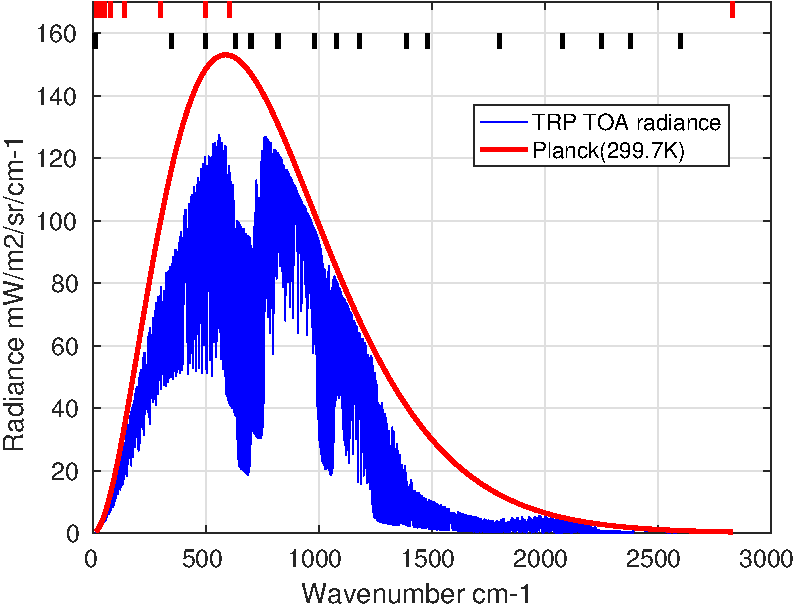
\includegraphics[width=0.625\textwidth]{Figs/generic_planckTOArads.pdf}
  \end{center}
  
  \begin{itemize}  
  \item Red hashlines : kCARTA band edges
  \item FarIR is a mix of H2004, H2008, H2012, MT-CKD 1
  \item Cannot really do Far IR cloud calcs
  \item so use RRTM (black hashlines : RRTM band edges)
  \end{itemize}

\end{frame}
% ---------------------------------------------------------------------
\begin{frame}
  \frametitle{kCARTA TOA BT (TRP profile)}

  \begin{center}
    \noindent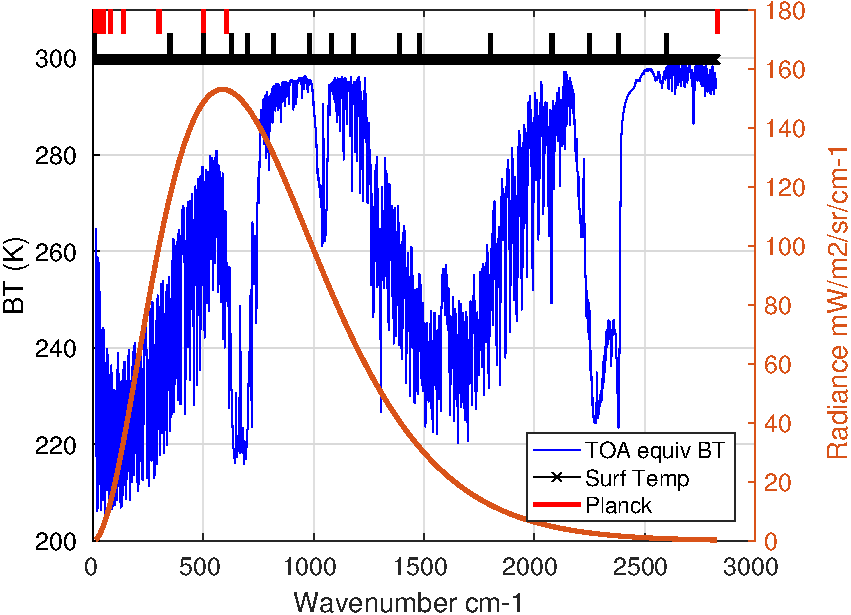
\includegraphics[width=0.95\textwidth]{Figs/generic_planckTOABT.pdf}
  \end{center}
  
\end{frame}
% ---------------------------------------------------------------------
\begin{frame}
  \frametitle{Comparing TOA radiances and Fluxes}

  \hspace{0.50in} TOA BT1231 \hspace{1.75in} Fluxes \\
  \begin{center}
    \dlandgraph{0.48}{Figs/generic_BT1231_vs_lat.pdf}{Figs/generic_olr_vs_lat.pdf}
  \end{center}

  \begin{itemize}
  \item Allsky radiance calcs use our TwoSlab clouds
    $r(\nu) = f_{ice} r_{ice}(\nu) + f_{water} r_{water}(\nu) +
    f_{overlap} r_{overlap}(\nu) + f_{clear} r_{clear}(\nu)$
  \item \textcolor{red}{So for now we try flux calcs using TwoSlab clouds!}
  \item RHS : 10 W/m2 CERES/TwoSlab bias, probably not emissivity
  \item LHS : BT231 is away from peak of Planck function, so lot of flux is absorbed by GHG
  \end{itemize}
\end{frame}
% ---------------------------------------------------------------------
% ---------------------------------------------------------------------
\section{Obs vs Calc}
% ---------------------------------------------------------------------
% ---------------------------------------------------------------------
\begin{frame}
  \frametitle{Obs and SARTA changes, BT1231}

  Earlier Larrabee showed BT1231 Sarta TwoSlab calcs are increasing by
  0.15 K/yr in the tropics, or $\sim$ 2.25 K over 15 years \newline

  \begin{columns}
    \begin{column}{0.65\columnwidth}
      \begin{center}
        \noindent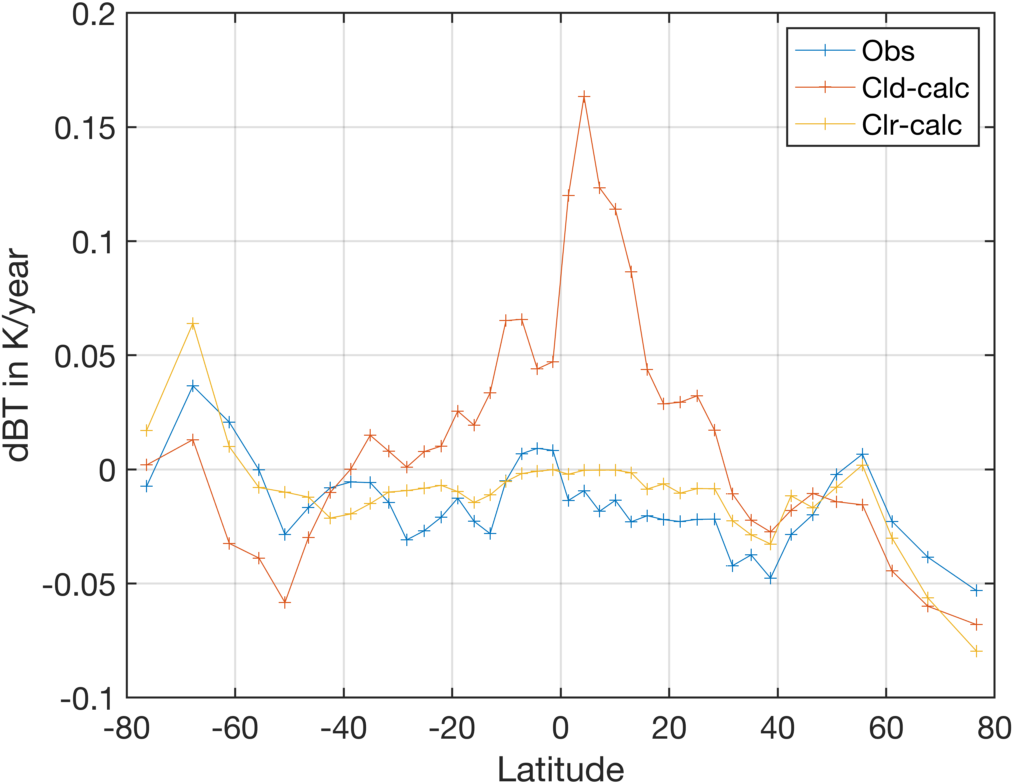
\includegraphics[width=\linewidth]{airs15year_lat_trends_900cm-1.png}
      \end{center}
    \end{column}

    \begin{column}{0.35\columnwidth}

      \vspace{0.1in}
      
      $dP = \sigma 4 T^3 dT$, with $T \sim 285 K, dT \sim 2.25 K $ $\rightarrow $
      \textcolor{red}{dP $\sim$ 11 W/m2} \newline

      That is not observed! \newline
      
      \vspace{0.1in}
      
      Can we understand where this comes from?

    \end{column}    
  \end{columns}
  
\end{frame}
% ---------------------------------------------------------------------
\begin{frame}
  \frametitle{Obs and SARTA changes, flux changes}

  \begin{center}
    \noindent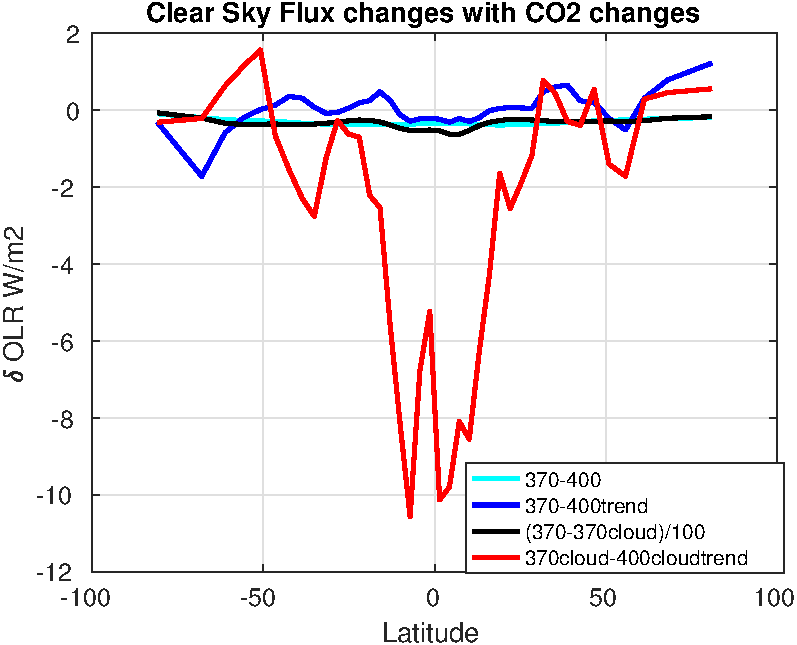
\includegraphics[width=0.375\textwidth]{Figs/deltaolr_vs_lat.pdf}
  \end{center}

  Take averaged profile over Year 01, all latbins, find OLR \newline
  Take averaged profile over Year 15, all latbins, find OLR \newline
  Turn on/off clouds, thermo, cloud, and CO2 changes
  \begin{itemize}
  \item Cyan : clear sky diff : CO2 trends
  \item Blue : clear sky diff : (CO2 + thermo + WV)trends
  \item Black : CO2 = 370 ppm; this is (clear sky vs cloudy sky)/100
  \item Red : allsky sky diff : (CO2 + thermo trends + WV trends + cloud) trends
  \end{itemize}
\end{frame}
% ---------------------------------------------------------------------
% ---------------------------------------------------------------------
\section{Flux Jacobians}
% ---------------------------------------------------------------------
% ---------------------------------------------------------------------
\begin{frame}
  \frametitle{Flux Jacobians : Method}
  \begin{itemize}
  \item Take daily zonal averages (AIRS obs, SARTA TwoSlab calcs, ERA thermodynamics + WV,O3)
  \item Do monthly averages (giving 180 between 2002/09 to 2017/08)
  \item Compute clear sky and TwoSlab fluxes for all latitude bins/180 months
  \item Add in CO2 change $\cd(t) = 370 + 2.2/12 \delta t$ where $\delta t = (t-2002/08)$ in months
  \item Now from this do yearly averages, in particular 2002/09-2003/08 and 2016/09-2017/08
  \item Call them Y1, Y15; take the yearly averaged profiles and keep doing fluxes as one parameter
    changes, with all other parameters held constant; \textcolor{red}{these are our 15 year jacobians}
  \end{itemize}
\end{frame}
% ---------------------------------------------------------------------
\begin{frame}
  \frametitle{Clear Sky Flux Jacobians}
  Changes are 2002/2003 to 2016/2017
  \begin{center}
    \noindent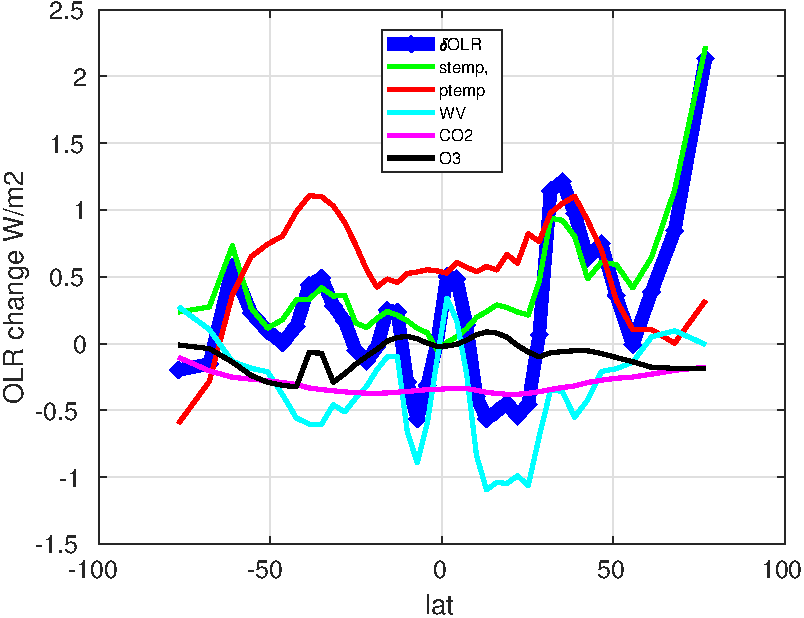
\includegraphics[width=0.5\linewidth]{Figs//clrsky_temp_gas_fluxjacs.pdf}
  \end{center}
  \begin{itemize}
  \item \cd (magenta),\water (cyan) increased, so flux is trapped
  \item surface, atmospheric temperatures (green and red) have also increased (more emission)
  \item so net change (BLUE with circles) is the combo of the above
  \end{itemize}
\end{frame}
% ---------------------------------------------------------------------
\begin{frame}
  \frametitle{All Sky Flux Jacobians}
  Changes are 2002/2003 to 2016/2017  \newline
  \hspace{0.50in} Thermodynamics \hspace{1.75in} Clouds \\
  \begin{center}
    \dlandgraph{0.48}{Figs//allsky_temp_gas_fluxjacs.pdf}{Figs//allsky_cloud_fluxjacs.pdf}
  \end{center}
  \begin{itemize}
  \item left panel clearly shows allsky flux changes (blue) is dominated by cloud changes (cyan)
  \item right panel shows the bulk of the increase in tropics is due to changes in ice cloud fraction!
  \end{itemize}  
\end{frame}
% ---------------------------------------------------------------------
% ---------------------------------------------------------------------
\section{Time series}
% ---------------------------------------------------------------------
% ---------------------------------------------------------------------
\begin{frame}
  \frametitle{Calculated Time Series}
  Monthly from 2002/09 to 2017/08 \newline
  \hspace{0.50in} Clear Sky  \hspace{1.75in} All Sky \\
  \begin{center}
    \dlandgraph{0.48}{Figs/olr_lat_time_nocloud.pdf}{Figs//olr_lat_time_cloud.pdf}
  \end{center}
\end{frame}
% ---------------------------------------------------------------------
\begin{frame}
  \frametitle{Greenhouse Effect}
  Monthly from 2002/09 to 2017/08 \newline
  We know monthly averaged surface temperatures so we know power emitted at surface, so we can compute GH effect (with clouds
  is larger than without clouds) \newline
  \hspace{0.50in} Clear Sky  \hspace{1.75in} All Sky \\
  \begin{center}
    \dlandgraph{0.48}{Figs/ghgeffect_delta_sb_olr_lat_time_nocloud.pdf}{Figs/ghgNcloudeffect_delta_sb_olr_lat_time.pdf}
  \end{center}
\end{frame}
% ---------------------------------------------------------------------
\begin{frame}
  \frametitle{Comparisons to CERES}
  \begin{center}
    \noindent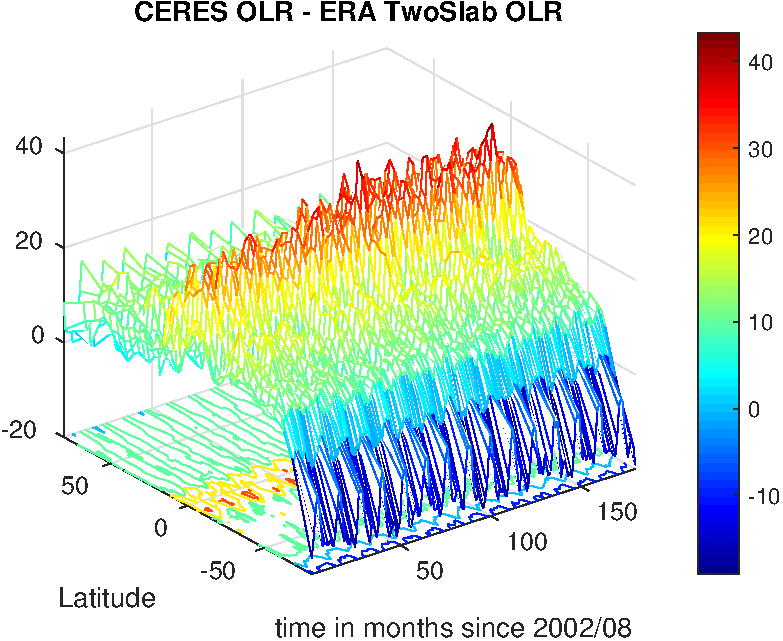
\includegraphics[width=0.75\linewidth]{Figs/ceresVSghgNcloudeffect_lat_time.pdf}
  \end{center}
  So clearly our implementation of TwoSlab/Fluxes is showing larger changes in OLR than are observed!
\end{frame}
% ---------------------------------------------------------------------
% ---------------------------------------------------------------------
\section{Flux Changes by RRTM bands}
% ---------------------------------------------------------------------
% ---------------------------------------------------------------------
\begin{frame}
  \frametitle{Flux Changes by RRTM bands}
  (2002/2003) - (2016/2017) : RED means MORE flux in 2002/2003 \newline
  \hspace{0.50in} Clear Sky  \hspace{1.75in} All Sky \\
  \begin{center}
    \dlandgraph{0.375}{Figs/spectral_deltaolr_vs_lat_thermo_gases.png}{Figs/spectral_deltaolr_vs_lat_thermo_gases_clouds.png}
  \end{center}

  \begin{small}
    \begin{itemize}
    \item LH panel, can see in 15 um band the change is red
    \item LH panel, can see more clr sky flux coming out in Southern Polar Regions in thermal window
    \item RH panel, more flux coming out in tropical window region in 2002
    \item RH panel, can see topical WV region had more flux emitted in 2002
    \end{itemize}
  \end{small}
\end{frame}
% ---------------------------------------------------------------------
% ---------------------------------------------------------------------
\section{Conclusions}
% ---------------------------------------------------------------------
% ---------------------------------------------------------------------
\begin{frame}
  \frametitle{Conclusions}
  \begin{itemize}
  \item RRTM allows us to dissect changes to OLR according to spectral region
  \item This gives us a different way to study climate trends
  \item TwoSlab fluxes "not too bad"!
  \item To do list : try MRO clouds in RRTM ....
  \item To do list : cloud changes from AIRS L1b spectral rates ...
  \end{itemize}
\end{frame}
% ---------------------------------------------------------------------
% ---------------------------------------------------------------------
\end{document}
% ---------------------------------------------------------------------
% ---------------------------------------------------------------------
